% Options for packages loaded elsewhere
\PassOptionsToPackage{unicode}{hyperref}
\PassOptionsToPackage{hyphens}{url}
%
\documentclass[
]{article}
\title{Moneyball - CUNY Data Science 621}
\author{Eric Hirsch}
\date{2/20/2021}

\usepackage{amsmath,amssymb}
\usepackage{lmodern}
\usepackage{iftex}
\ifPDFTeX
  \usepackage[T1]{fontenc}
  \usepackage[utf8]{inputenc}
  \usepackage{textcomp} % provide euro and other symbols
\else % if luatex or xetex
  \usepackage{unicode-math}
  \defaultfontfeatures{Scale=MatchLowercase}
  \defaultfontfeatures[\rmfamily]{Ligatures=TeX,Scale=1}
\fi
% Use upquote if available, for straight quotes in verbatim environments
\IfFileExists{upquote.sty}{\usepackage{upquote}}{}
\IfFileExists{microtype.sty}{% use microtype if available
  \usepackage[]{microtype}
  \UseMicrotypeSet[protrusion]{basicmath} % disable protrusion for tt fonts
}{}
\makeatletter
\@ifundefined{KOMAClassName}{% if non-KOMA class
  \IfFileExists{parskip.sty}{%
    \usepackage{parskip}
  }{% else
    \setlength{\parindent}{0pt}
    \setlength{\parskip}{6pt plus 2pt minus 1pt}}
}{% if KOMA class
  \KOMAoptions{parskip=half}}
\makeatother
\usepackage{xcolor}
\IfFileExists{xurl.sty}{\usepackage{xurl}}{} % add URL line breaks if available
\IfFileExists{bookmark.sty}{\usepackage{bookmark}}{\usepackage{hyperref}}
\hypersetup{
  pdftitle={Moneyball - CUNY Data Science 621},
  pdfauthor={Eric Hirsch},
  hidelinks,
  pdfcreator={LaTeX via pandoc}}
\urlstyle{same} % disable monospaced font for URLs
\usepackage[margin=1in]{geometry}
\usepackage{graphicx}
\makeatletter
\def\maxwidth{\ifdim\Gin@nat@width>\linewidth\linewidth\else\Gin@nat@width\fi}
\def\maxheight{\ifdim\Gin@nat@height>\textheight\textheight\else\Gin@nat@height\fi}
\makeatother
% Scale images if necessary, so that they will not overflow the page
% margins by default, and it is still possible to overwrite the defaults
% using explicit options in \includegraphics[width, height, ...]{}
\setkeys{Gin}{width=\maxwidth,height=\maxheight,keepaspectratio}
% Set default figure placement to htbp
\makeatletter
\def\fps@figure{htbp}
\makeatother
\setlength{\emergencystretch}{3em} % prevent overfull lines
\providecommand{\tightlist}{%
  \setlength{\itemsep}{0pt}\setlength{\parskip}{0pt}}
\setcounter{secnumdepth}{-\maxdimen} % remove section numbering
\ifLuaTeX
  \usepackage{selnolig}  % disable illegal ligatures
\fi

\begin{document}
\maketitle

\hypertarget{description-of-the-dataset}{%
\subsection{Description of the
Dataset}\label{description-of-the-dataset}}

xxxxxx

\hypertarget{data-exploration}{%
\subsubsection{Data Exploration}\label{data-exploration}}

summary info

\begin{verbatim}
##      INDEX         TARGET_WINS       BATTING_H      BATTING_2B   
##  Min.   :   1.0   Min.   :  0.00   Min.   : 891   Min.   : 69.0  
##  1st Qu.: 630.8   1st Qu.: 71.00   1st Qu.:1383   1st Qu.:208.0  
##  Median :1270.5   Median : 82.00   Median :1454   Median :238.0  
##  Mean   :1268.5   Mean   : 80.79   Mean   :1469   Mean   :241.2  
##  3rd Qu.:1915.5   3rd Qu.: 92.00   3rd Qu.:1537   3rd Qu.:273.0  
##  Max.   :2535.0   Max.   :146.00   Max.   :2554   Max.   :458.0  
##                                                                  
##    BATTING_3B       BATTING_HR       BATTING_BB      BATTING_SO    
##  Min.   :  0.00   Min.   :  0.00   Min.   :  0.0   Min.   :   0.0  
##  1st Qu.: 34.00   1st Qu.: 42.00   1st Qu.:451.0   1st Qu.: 548.0  
##  Median : 47.00   Median :102.00   Median :512.0   Median : 750.0  
##  Mean   : 55.25   Mean   : 99.61   Mean   :501.6   Mean   : 735.6  
##  3rd Qu.: 72.00   3rd Qu.:147.00   3rd Qu.:580.0   3rd Qu.: 930.0  
##  Max.   :223.00   Max.   :264.00   Max.   :878.0   Max.   :1399.0  
##                                                    NA's   :102     
##    BASERUN_SB      BASERUN_CS     BATTING_HBP      PITCHING_H   
##  Min.   :  0.0   Min.   :  0.0   Min.   :29.00   Min.   : 1137  
##  1st Qu.: 66.0   1st Qu.: 38.0   1st Qu.:50.50   1st Qu.: 1419  
##  Median :101.0   Median : 49.0   Median :58.00   Median : 1518  
##  Mean   :124.8   Mean   : 52.8   Mean   :59.36   Mean   : 1779  
##  3rd Qu.:156.0   3rd Qu.: 62.0   3rd Qu.:67.00   3rd Qu.: 1682  
##  Max.   :697.0   Max.   :201.0   Max.   :95.00   Max.   :30132  
##  NA's   :131     NA's   :772     NA's   :2085                   
##   PITCHING_HR     PITCHING_BB      PITCHING_SO        FIELDING_E    
##  Min.   :  0.0   Min.   :   0.0   Min.   :    0.0   Min.   :  65.0  
##  1st Qu.: 50.0   1st Qu.: 476.0   1st Qu.:  615.0   1st Qu.: 127.0  
##  Median :107.0   Median : 536.5   Median :  813.5   Median : 159.0  
##  Mean   :105.7   Mean   : 553.0   Mean   :  817.7   Mean   : 246.5  
##  3rd Qu.:150.0   3rd Qu.: 611.0   3rd Qu.:  968.0   3rd Qu.: 249.2  
##  Max.   :343.0   Max.   :3645.0   Max.   :19278.0   Max.   :1898.0  
##                                   NA's   :102                       
##   FIELDING_DP   
##  Min.   : 52.0  
##  1st Qu.:131.0  
##  Median :149.0  
##  Mean   :146.4  
##  3rd Qu.:164.0  
##  Max.   :228.0  
##  NA's   :286
\end{verbatim}

Histograms
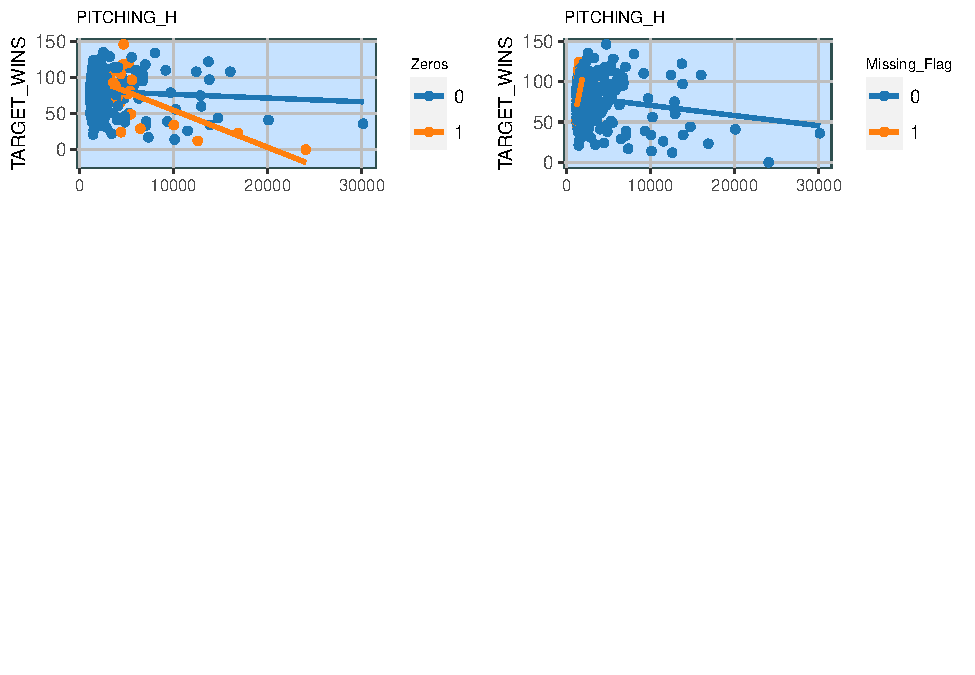
\includegraphics{Baseball_tmp_files/figure-latex/unnamed-chunk-13-1.pdf}

boxplots and correlations

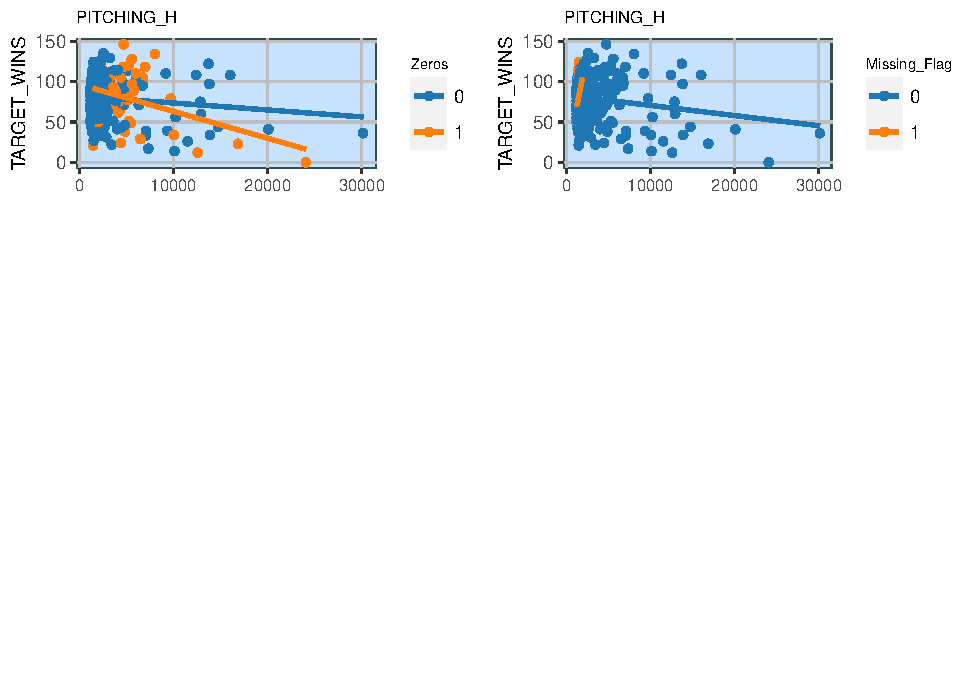
\includegraphics{Baseball_tmp_files/figure-latex/unnamed-chunk-14-1.pdf}

dealing with outliers

correlations:

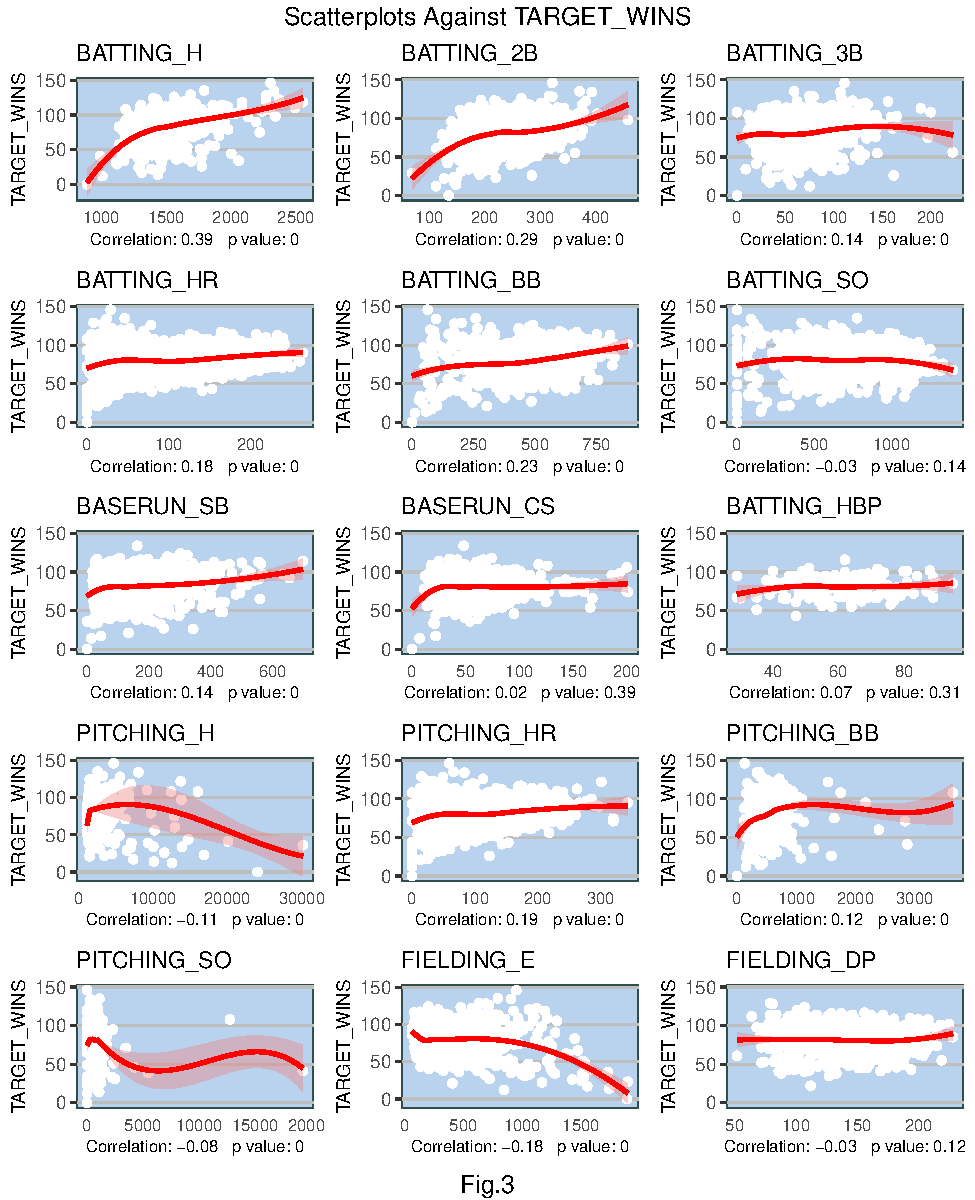
\includegraphics{Baseball_tmp_files/figure-latex/fig-1.pdf}

looking at mutlicollinearlity

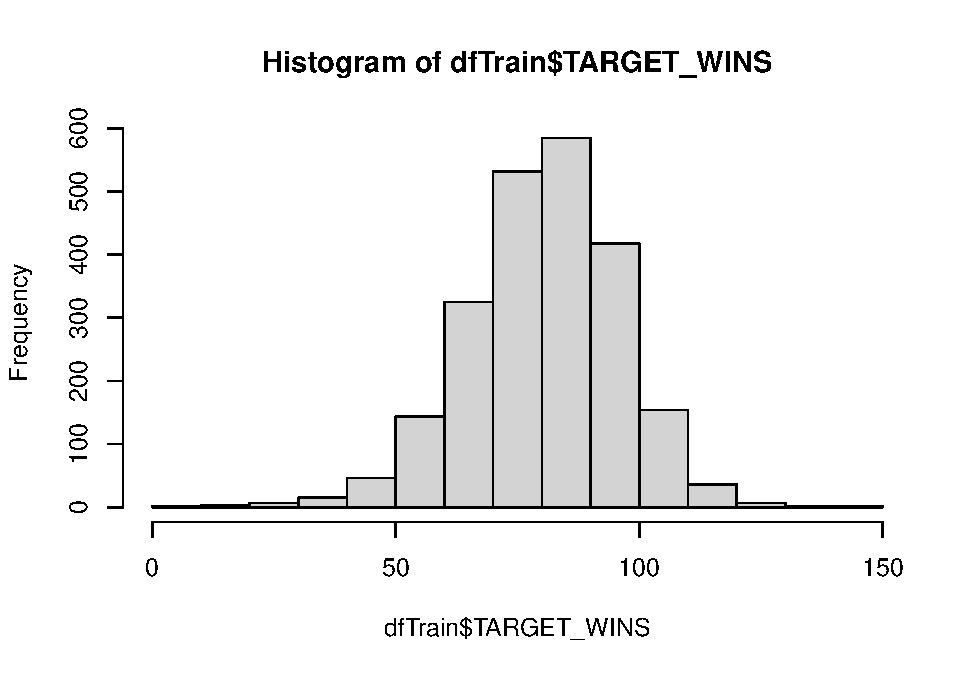
\includegraphics{Baseball_tmp_files/figure-latex/unnamed-chunk-15-1.pdf}

Examine dependent variable

\hypertarget{data-preparation}{%
\subsubsection{Data Preparation}\label{data-preparation}}

Dealing with na - get rid of hbp and cs, create flags, check if
Batting\_SO is random

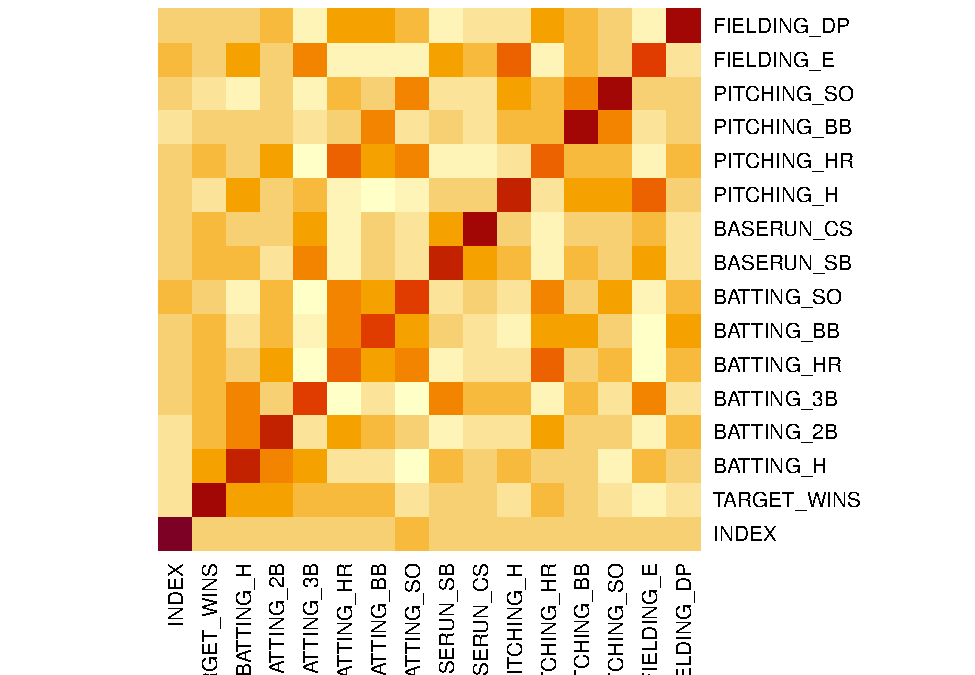
\includegraphics{Baseball_tmp_files/figure-latex/unnamed-chunk-16-1.pdf}

Imputation missing values

\begin{verbatim}
## [1] "type:" "mean" 
## [1] "r2mean:" "0.4074" 
## [1] "r2median:" "0.4074"   
## [1] "r2omit" "0.4019"
\end{verbatim}

\begin{verbatim}
## [1] "type:" "mean" 
## [1] "r2mean:" "0.4074" 
## [1] "r2median:" "0.4074"   
## [1] "r2omit" "0.4019"
\end{verbatim}

Transformations: . Here we only look at \textless=300 to get better idea
of starnge area pitching\_h - deal with odd behavior

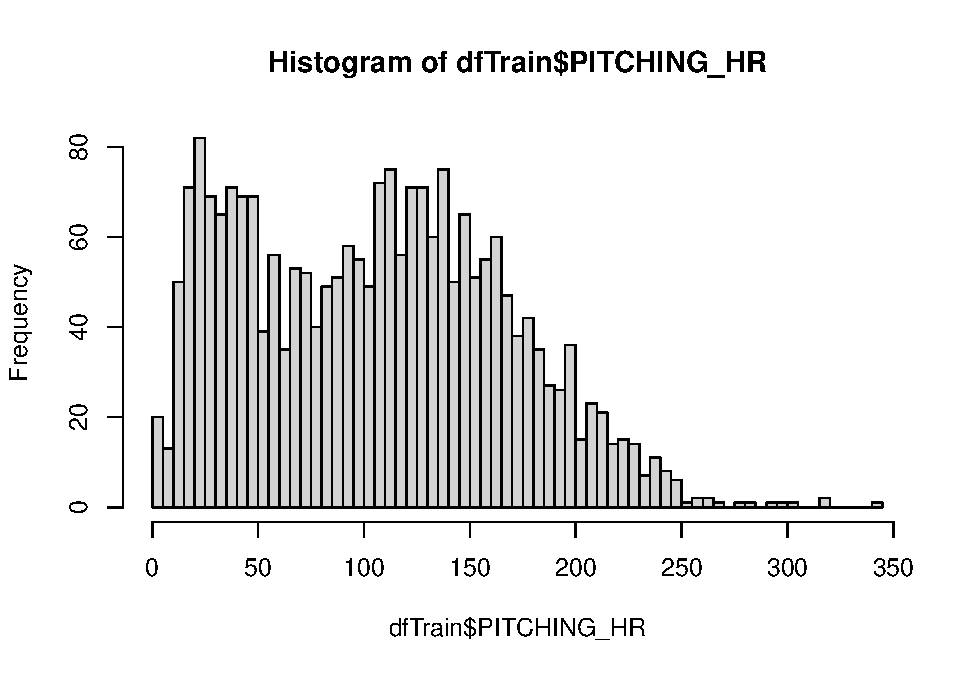
\includegraphics{Baseball_tmp_files/figure-latex/unnamed-chunk-18-1.pdf}

F\_DP - deal with relationship to hits

\begin{verbatim}
## [1] 0.0003924305
\end{verbatim}

\begin{verbatim}
## [1] 0.01398409
\end{verbatim}

\begin{verbatim}
## [1] 0.02142144
\end{verbatim}

Home runs - deal with implausibility (drop pitch)

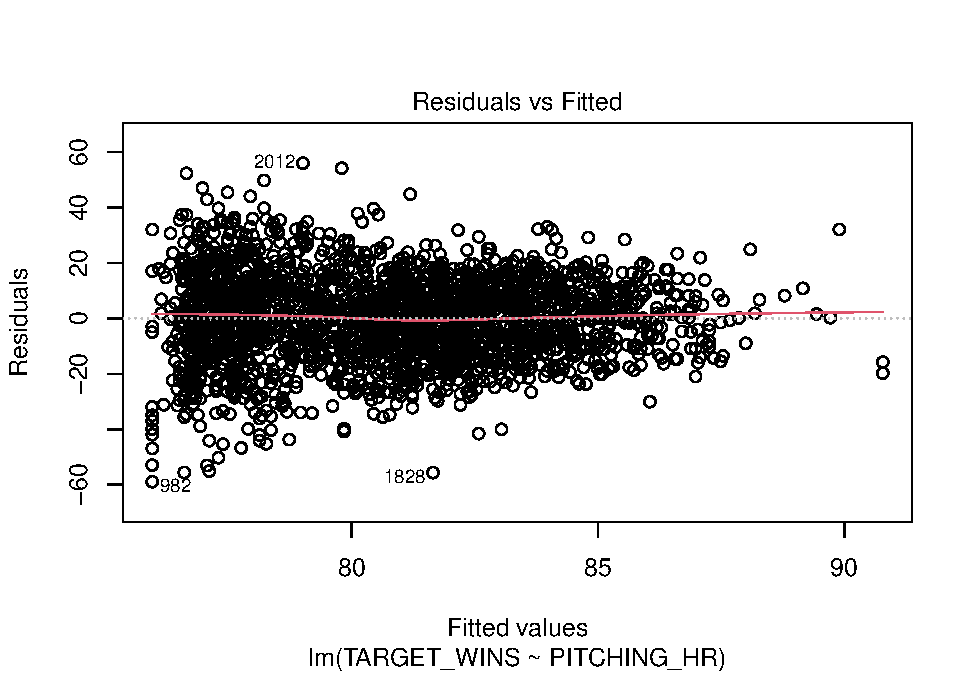
\includegraphics{Baseball_tmp_files/figure-latex/unnamed-chunk-20-1.pdf}
deal with bimodaility(create HR under 60)

\begin{verbatim}
## [1] 0.03060384
\end{verbatim}

\begin{verbatim}
## [1] 0.03617586
\end{verbatim}

create new errors field

\begin{verbatim}
## [1] 0.03072081
\end{verbatim}

\begin{verbatim}
## [1] 0.04825783
\end{verbatim}

Create Missing ``cohort'' interactions

\hypertarget{build-models}{%
\subsubsection{Build Models}\label{build-models}}

Create regression 1 - no transformations except missing flags

\begin{verbatim}
## 
## Call:
## lm(formula = TARGET_WINS ~ BATTING_H + BATTING_2B + BATTING_3B + 
##     BATTING_HR + BATTING_BB + BATTING_SO + BASERUN_SB + PITCHING_H + 
##     PITCHING_SO + FIELDING_E + FIELDING_DP + BSO_Missing_Flag + 
##     BRSB_Missing_Flag + FDP_Missing_Flag, data = df)
## 
## Residuals:
##     Min      1Q  Median      3Q     Max 
## -63.849  -7.994   0.338   7.926  49.898 
## 
## Coefficients:
##                     Estimate Std. Error t value Pr(>|t|)    
## (Intercept)       20.7188116  5.1141823   4.051 5.27e-05 ***
## BATTING_H          0.0481387  0.0034185  14.082  < 2e-16 ***
## BATTING_2B        -0.0357462  0.0086576  -4.129 3.78e-05 ***
## BATTING_3B         0.0550541  0.0155444   3.542 0.000406 ***
## BATTING_HR         0.0711042  0.0091701   7.754 1.34e-14 ***
## BATTING_BB         0.0253016  0.0032449   7.797 9.58e-15 ***
## BATTING_SO        -0.0107507  0.0023244  -4.625 3.95e-06 ***
## BASERUN_SB         0.0497807  0.0046076  10.804  < 2e-16 ***
## PITCHING_H         0.0019828  0.0003352   5.916 3.81e-09 ***
## PITCHING_SO       -0.0009736  0.0006627  -1.469 0.141921    
## FIELDING_E        -0.0570291  0.0033828 -16.859  < 2e-16 ***
## FIELDING_DP       -0.1003640  0.0134425  -7.466 1.17e-13 ***
## BSO_Missing_Flag   8.7007564  1.4580508   5.967 2.79e-09 ***
## BRSB_Missing_Flag 33.7150508  1.8190459  18.534  < 2e-16 ***
## FDP_Missing_Flag   4.2670950  1.4589567   2.925 0.003482 ** 
## ---
## Signif. codes:  0 '***' 0.001 '**' 0.01 '*' 0.05 '.' 0.1 ' ' 1
## 
## Residual standard error: 12.13 on 2261 degrees of freedom
## Multiple R-squared:  0.411,  Adjusted R-squared:  0.4074 
## F-statistic: 112.7 on 14 and 2261 DF,  p-value: < 2.2e-16
## 
## [1] "VIF Analysis"
##         BATTING_H        BATTING_2B        BATTING_3B        BATTING_HR 
##          3.779947          2.540104          2.918055          4.769509 
##        BATTING_BB        BATTING_SO        BASERUN_SB        PITCHING_H 
##          2.451529          4.931438          2.385757          3.440215 
##       PITCHING_SO        FIELDING_E       FIELDING_DP  BSO_Missing_Flag 
##          1.985417          9.184956          1.681234          1.408612 
## BRSB_Missing_Flag  FDP_Missing_Flag 
##          2.778256          3.619847
\end{verbatim}

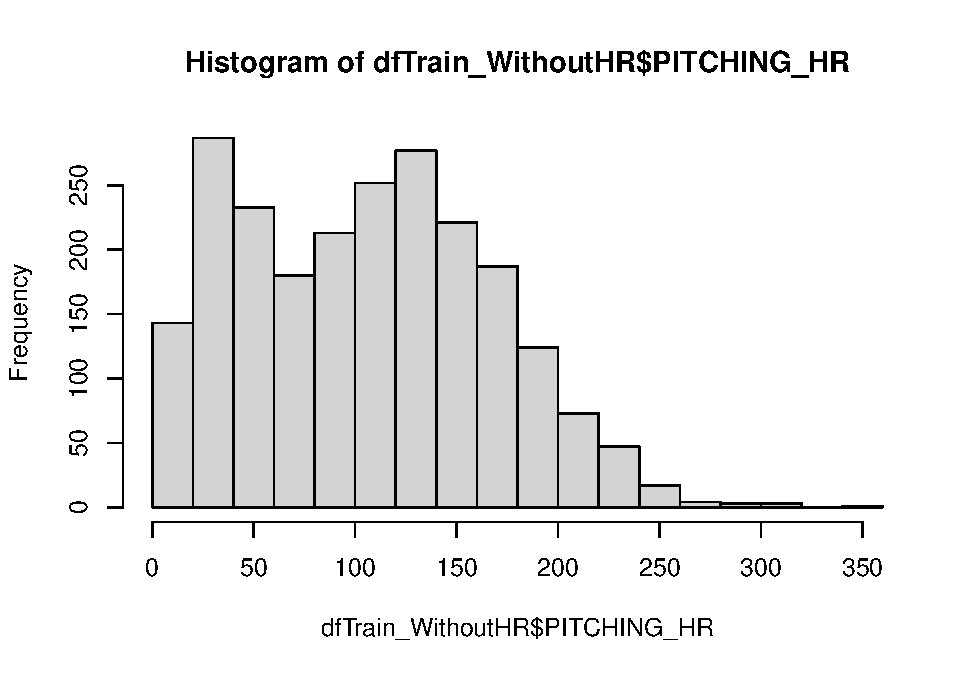
\includegraphics{Baseball_tmp_files/figure-latex/unnamed-chunk-24-1.pdf}

\begin{verbatim}
## NULL
\end{verbatim}

Model 2, all the transformations:

\begin{verbatim}
## 
## Call:
## lm(formula = TARGET_WINS ~ BATTING_H + BATTING_2B + BATTING_3B + 
##     BATTING_HR + BATTING_BB + BATTING_SO + BASERUN_SB + PITCHING_H + 
##     FIELDING_E + FIELDING_DP + BSO_Missing_Flag + BRSB_Missing_Flag + 
##     FDP_Missing_Flag + Pitch_h_Under1500 + E_sq + Inter_E_Cohort + 
##     Inter_bhr_Cohort + Inter_bs_Cohort, data = df)
## 
## Residuals:
##     Min      1Q  Median      3Q     Max 
## -52.914  -7.727   0.159   7.657  49.775 
## 
## Coefficients:
##                     Estimate Std. Error t value Pr(>|t|)    
## (Intercept)        2.036e+01  5.340e+00   3.812 0.000141 ***
## BATTING_H          5.197e-02  3.369e-03  15.428  < 2e-16 ***
## BATTING_2B        -3.576e-02  8.564e-03  -4.176 3.08e-05 ***
## BATTING_3B         7.470e-02  1.573e-02   4.749 2.17e-06 ***
## BATTING_HR         6.411e-02  9.163e-03   6.997 3.44e-12 ***
## BATTING_BB         2.574e-02  3.186e-03   8.079 1.05e-15 ***
## BATTING_SO        -1.307e-02  2.163e-03  -6.046 1.74e-09 ***
## BASERUN_SB         5.110e-02  4.674e-03  10.934  < 2e-16 ***
## PITCHING_H         1.020e-03  2.955e-04   3.452 0.000566 ***
## FIELDING_E        -8.132e-02  7.033e-03 -11.563  < 2e-16 ***
## FIELDING_DP       -1.063e-01  1.333e-02  -7.972 2.46e-15 ***
## BSO_Missing_Flag   4.677e+01  9.614e+00   4.864 1.23e-06 ***
## BRSB_Missing_Flag  3.562e+01  1.855e+00  19.204  < 2e-16 ***
## FDP_Missing_Flag   6.209e+00  1.507e+00   4.119 3.94e-05 ***
## Pitch_h_Under1500  2.018e+00  6.760e-01   2.985 0.002864 ** 
## E_sq               1.897e-05  4.097e-06   4.631 3.85e-06 ***
## Inter_E_Cohort    -1.801e-01  2.620e-02  -6.874 8.05e-12 ***
## Inter_bhr_Cohort   3.514e-01  1.515e-01   2.320 0.020404 *  
## Inter_bs_Cohort    4.870e-02  2.397e-02   2.032 0.042287 *  
## ---
## Signif. codes:  0 '***' 0.001 '**' 0.01 '*' 0.05 '.' 0.1 ' ' 1
## 
## Residual standard error: 11.87 on 2257 degrees of freedom
## Multiple R-squared:  0.437,  Adjusted R-squared:  0.4325 
## F-statistic: 97.34 on 18 and 2257 DF,  p-value: < 2.2e-16
## 
## [1] "VIF Analysis"
##         BATTING_H        BATTING_2B        BATTING_3B        BATTING_HR 
##          3.833033          2.595576          3.120382          4.973356 
##        BATTING_BB        BATTING_SO        BASERUN_SB        PITCHING_H 
##          2.468116          4.457772          2.563766          2.792528 
##        FIELDING_E       FIELDING_DP  BSO_Missing_Flag BRSB_Missing_Flag 
##         41.459797          1.726987         63.952655          3.017211 
##  FDP_Missing_Flag Pitch_h_Under1500              E_sq    Inter_E_Cohort 
##          4.035107          1.833498         22.339941         44.481566 
##  Inter_bhr_Cohort   Inter_bs_Cohort 
##          7.360403         17.564481
\end{verbatim}

\includegraphics{Baseball_tmp_files/figure-latex/unnamed-chunk-25-1.pdf}

\begin{verbatim}
## NULL
\end{verbatim}

second model explains better, but does not necessarily perform lot
better.

Third model, categories of power - batting power and pitching weakness

categories

The two are correlated

\begin{verbatim}
## [1] 0.3967352
\end{verbatim}

These boxplots show the stronger relationship with batting power

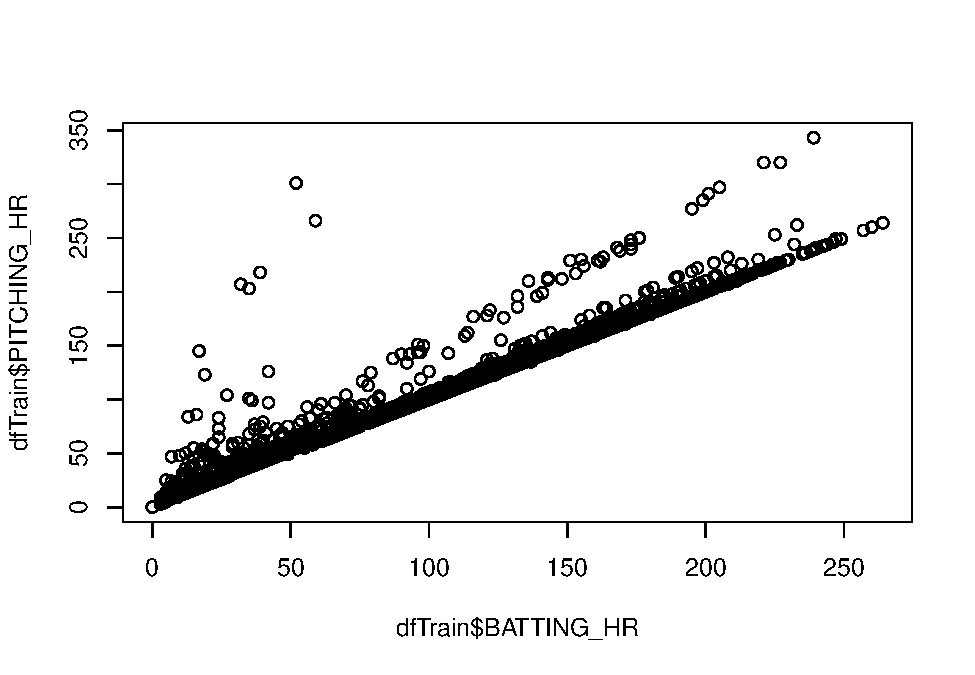
\includegraphics{Baseball_tmp_files/figure-latex/unnamed-chunk-28-1.pdf}

we run the regressions

\begin{verbatim}
## 
## Call:
## lm(formula = TARGET_WINS ~ Total_Power, data = dfCat)
## 
## Residuals:
##     Min      1Q  Median      3Q     Max 
## -74.784 -10.648   1.216  10.333  63.294 
## 
## Coefficients:
##             Estimate Std. Error t value Pr(>|t|)    
## (Intercept)  82.7062     0.4841 170.840   <2e-16 ***
## Total_Power   1.9804     0.2154   9.196   <2e-16 ***
## ---
## Signif. codes:  0 '***' 0.001 '**' 0.01 '*' 0.05 '.' 0.1 ' ' 1
## 
## Residual standard error: 16.78 on 1200 degrees of freedom
## Multiple R-squared:  0.06583,    Adjusted R-squared:  0.06505 
## F-statistic: 84.57 on 1 and 1200 DF,  p-value: < 2.2e-16
\end{verbatim}

\begin{verbatim}
## 
## Call:
## lm(formula = TARGET_WINS ~ Hitting_Power + Pitching_Weakness, 
##     data = dfCat)
## 
## Residuals:
##     Min      1Q  Median      3Q     Max 
## -68.817  -9.239   0.898  10.008  63.261 
## 
## Coefficients:
##                   Estimate Std. Error t value Pr(>|t|)    
## (Intercept)        64.2645     1.6750  38.367   <2e-16 ***
## Hitting_Power       3.4805     0.2429  14.328   <2e-16 ***
## Pitching_Weakness  -0.4014     0.2467  -1.627    0.104    
## ---
## Signif. codes:  0 '***' 0.001 '**' 0.01 '*' 0.05 '.' 0.1 ' ' 1
## 
## Residual standard error: 15.94 on 1199 degrees of freedom
## Multiple R-squared:  0.1579, Adjusted R-squared:  0.1565 
## F-statistic: 112.4 on 2 and 1199 DF,  p-value: < 2.2e-16
\end{verbatim}

\begin{verbatim}
## 
## Call:
## lm(formula = TARGET_WINS ~ category_PH + category_PBB + category_BH + 
##     category_BBB + category_BHR, data = dfCat)
## 
## Residuals:
##     Min      1Q  Median      3Q     Max 
## -68.963  -9.135   0.638  10.306  61.786 
## 
## Coefficients:
##              Estimate Std. Error t value Pr(>|t|)    
## (Intercept)   60.8092     2.0524  29.628  < 2e-16 ***
## category_PH    0.2114     0.4858   0.435 0.663612    
## category_PBB  -0.3393     0.6446  -0.526 0.598735    
## category_BH    3.8127     0.3891   9.799  < 2e-16 ***
## category_BBB   2.2187     0.7112   3.119 0.001855 ** 
## category_BHR   1.4053     0.4252   3.305 0.000977 ***
## ---
## Signif. codes:  0 '***' 0.001 '**' 0.01 '*' 0.05 '.' 0.1 ' ' 1
## 
## Residual standard error: 15.83 on 1196 degrees of freedom
## Multiple R-squared:  0.1714, Adjusted R-squared:  0.1679 
## F-statistic: 49.46 on 5 and 1196 DF,  p-value: < 2.2e-16
\end{verbatim}

Analysis shows good batting and weak pitching are correlated. Poor r
squared but significant batting.

\hypertarget{select-models}{%
\subsubsection{Select models}\label{select-models}}

Now we make predictions

\end{document}
